% Created 2026-02-04 Wed 17:29
% Intended LaTeX compiler: pdflatex
\documentclass{ieeeqccl}
\usepackage[utf8]{inputenc}
\usepackage[T1]{fontenc}
\usepackage{graphicx}
\usepackage{longtable}
\usepackage{wrapfig}
\usepackage{rotating}
\usepackage[normalem]{ulem}
\usepackage{amsmath}
\usepackage{amssymb}
\usepackage{capt-of}
\usepackage{hyperref}
\usepackage{subcaption}
\usepackage[backend=biber]{biblatex}
\addbibresource{/home/amitav-krishna/qnr/wip/references.bib}
\addbibresource{references.bib}
\usepackage[font=small,labelfont=bf]{caption}
\captionsetup{list=no}
\author{Amitav Krishna\thanks{Correspondence: amitavkrishna@proton.me}}
\date{\today}
\title{Frobenius Normalization Enables Stable Training for Quantum State Denoising}
\hypersetup{
 pdfauthor={Amitav Krishna\thanks{Correspondence: amitavkrishna@proton.me}},
 pdftitle={Frobenius Normalization Enables Stable Training for Quantum State Denoising},
 pdfkeywords={},
 pdfsubject={},
 pdfcreator={Emacs 29.3 (Org mode 9.6.15)}, 
 pdflang={English}}
\begin{document}

\maketitle

\section{Abstract}
\label{sec:org36157be}
Quantum computerspenis penis penis penis penis penis penis penis penis penis penis penis penis penis penis penis penis penis penis penis penis penis penis penis penis  offer asymptotic speedups for problems like molecular simulation and integer factorization, but noise severely limits their near-term utility.  Quantum Error Correction can address this, but the number of extra qubits required makes it infeasible for near-term use while the cost per qubit remains high.  Quantum Error Mitigation is a near-term alternative, but only recovers expectation values, not the full quantum state needed for extracting accurate results from simulations run on quantum hardware.  For these, we need quantum state reconstruction.  Quantum state tomography estimates a state by measuring the system across many bases, but these measurements are inherently noisy; quantum state reconstruction recovers a clean density matrix from this noisy data.  Neural networks have shown promise here, but previous work has only been demonstrated up to 5 qubits.  We find that Frobenius normalization (scaling inputs to unit purity) removes this bottleneck, enabling scaling to 8-qubit systems while maintaining a  relatively large improvement in fidelity. 
\section{Introduction}
\label{sec:org82ab605}
Quantum computers hold the potential to enable exponential speedups of many tasks through their exploitation of the principles of quantum mechanics \autocite{feynman1982simulating}, specifically the ability to explore possibilities in superposition, with paths that interfere to amplify correct answers and cancel wrong ones. However, this interference is both a blessing and a curse. After enough time, the computer will inevitably become fully entangled with the environment, locking the information in correlations with the rest of the universe and throwing away the key, leaving us, the observers, with nothing to work with.nnn

\begin{figure}[!t]
\centering
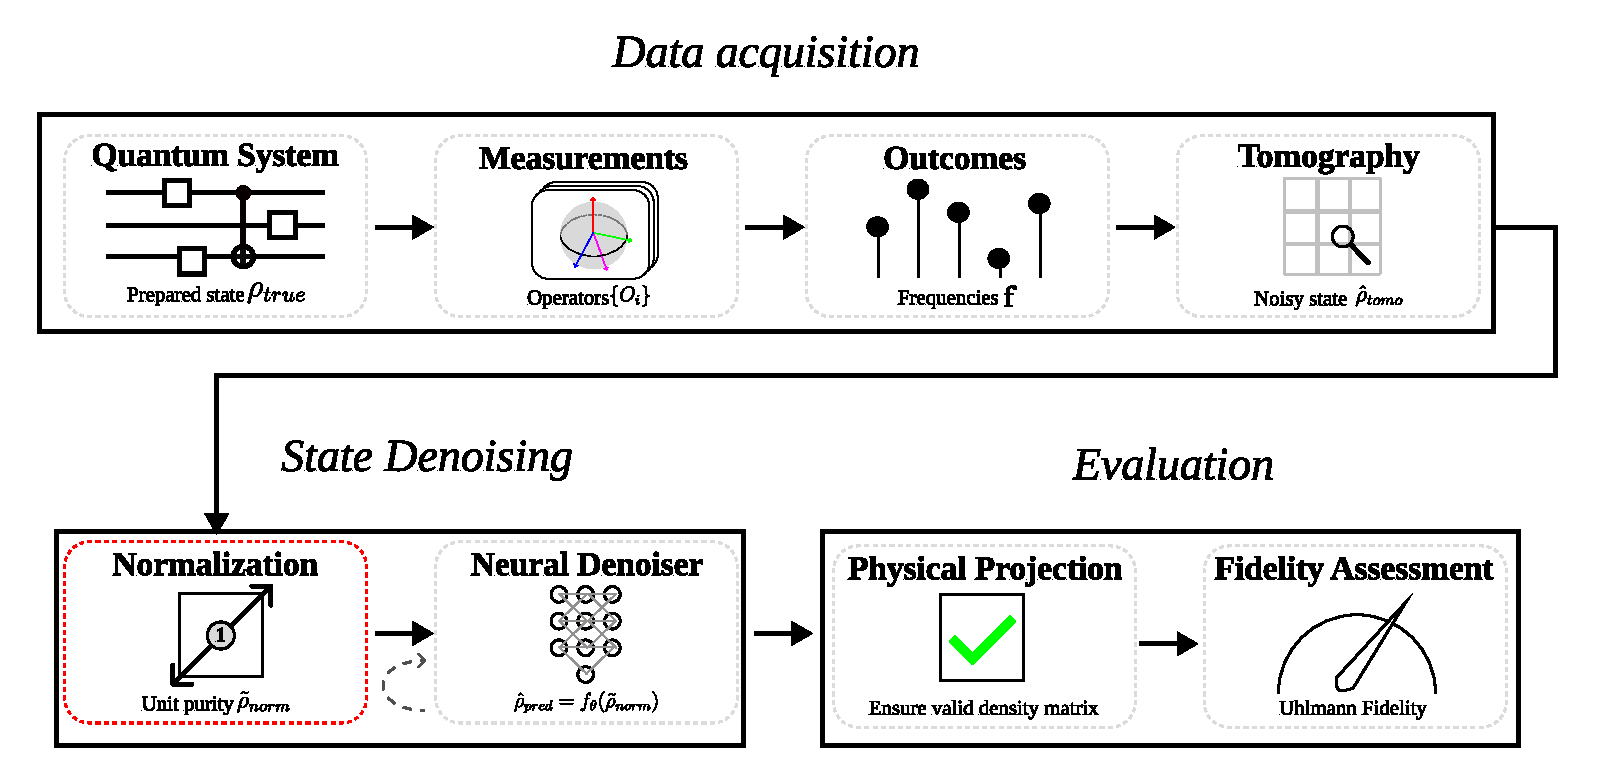
\includegraphics[width=\columnwidth]{figures/QEM Process diagram (2).pdf}
\caption{\label{fig:orgea48f15}Overview of the training and evaluation pipeline. Quantum states are measured, reconstructed via tomography, and normalized to unit Frobenius norm. A neural denoiser maps the normalized noisy state to a denoised estimate, which is then projected to a valid density matrix before computing Uhlmann fidelity.}
\end{figure}

Quantum Error Correction addresses this by encoding a single logical qubit on multiple physical qubits, and then using ancillary qubits to detect errors. To detect errors, we check whether pairs of data qubits match, entangling the ancilla with just this parity information. Crucially, we do not entangle the ancilla with the data itself, so measuring the ancilla only collapses the parity, not the data itself, which stays in superposition. Measuring the bitstring of the ancilla gives us the syndrome, which is then decoded on a classical computer to find the necessary correction. While QEC is a scalable, principled method to reducing errors in quantum computers, useful error rates require on the order of \textasciitilde{}1,000+ physical qubits per logical qubit \autocite{2024}, making it infeasible for the near-term \autocite{preskill2018quantum}.

Quantum Error Mitigation, on the other hand, is a method to reducing quantum noise in the short term \autocite{RevModPhys.95.045005}. QEM requires no extra qubits, and instead runs corrections classically. Common techniques include zero-noise extrapolation, where one runs a circuit multiple times with artificially increased noise levels and extrapolates back to zero noise, and probabilistic error cancellation, which inserts random operations that statistically average out the noise. However, QEM only recovers expectation values—single numbers like ⟨Z⟩—not the full quantum state. For tasks that require the complete density matrix, such as verifying entanglement or extracting detailed simulation results, expectation values are not enough.

Quantum State Reconstruction addresses this gap. Like QEM, it uses classical post-processing and requires no extra qubits. But instead of recovering expectation values, QSR recovers the full density matrix from noisy tomographic data. Recent work has shown that neural networks can learn to invert noise channels, taking a noisy density matrix and outputting a denoised estimate \autocite{Morgillo_2024,kendre2025machinelearningquantumnoise,Torlai2018}. However, previous neural network approaches have only been demonstrated up to 5 qubits. We introduce a data normalization method that removes this bottleneck, enabling scaling to 8-qubit systems.

We generate synthetic datasets by simulating random quantum circuits composed of single-qubit gates (X, Y, Z, H, rotations) and two-qubit entangling gates (CNOT, CZ, SWAP). Each circuit is simulated twice: once ideally to produce a clean density matrix, and once with noise channels (depolarizing, amplitude damping, phase damping, bit flip) applied after each layer to produce a noisy counterpart. We train neural networks to map noisy inputs to clean targets, using Frobenius fidelity as the loss function. The key preprocessing step is Frobenius normalization: we scale each density matrix to unit norm before training. The Frobenius norm of a density matrix equals the square root of its purity—a measure of how "purely quantum" vs. "classically mixed" the state is. Since noisy states have norms significantly smaller than clean states—up to \textasciitilde{}16× for 8-qubit systems (a physical consequence of decoherence pushing states toward the maximally mixed state)—this normalization decouples scale recovery from structural denoising, allowing the model to focus on restoring coherence structure rather than learning a global rescaling.

On 5-qubit systems, normalization reduces validation loss by 25\% and enables both MLP and Transformer architectures to achieve >3 times improvement in Uhlmann fidelity over the noisy baseline. Without normalization, scaling model capacity actually hurts performance—a signature of optimization pathology. On 8-qubit systems (\(256 \times 256\) density matrices), training without normalization fails entirely, while normalized models achieve 3–4 times improvement over baseline. Our results suggest that for neural QSR, input conditioning matters more than architectural choice, as both MLPs and Transformers achieve similar performance once properly normalized. The scale mismatch caused by decoherence is a domain-specific challenge that requires domain-specific preprocessing, and we recommend Frobenius normalization as a standard step for any neural approach to quantum state reconstruction.

Section 2 reviews related work on input normalization and neural approaches to quantum error correction. Section 3 describes our dataset generation, model architectures, and the Frobenius normalization method. Section 4 presents our experimental results. Section 5 discusses the physical interpretation and limitations of our approach. Section 6 concludes.
\section{Related Work}
\label{sec:org121c088}

Input normalization is well-established in deep learning. Batch normalization \autocite{ioffe2015batch} and layer normalization \autocite{ba2016layer} address internal covariate shift, while input standardization (zero mean, unit variance) is standard practice for feedforward networks. However, quantum density matrices present a unique challenge: the \textbf{inherent} scale difference between noisy and clean states is not statistical variation but a physical consequence of decoherence. Our work identifies Frobenius normalization as the appropriate preprocessing for this domain, demonstrating that it is not merely helpful but \textbf{essential} for stable training and scaling at larger scales.

Machine learning has been widely applied to quantum error correction (QEC). Recent work such as Transformer-QEC \autocite{wang2023transformerqecquantumerrorcorrection} demonstrates that attention mechanisms outperform local decoders (like CNNs) for syndrome decoding by capturing non-local error chains. Work by Morgillo et al. \autocite{Morgillo_2024} and Kendre et al. \autocite{kendre2025machinelearningquantumnoise} has explored neural approaches to quantum state reconstruction, though without addressing the input normalization challenge we identify here.

For computational tractability at larger qubit counts, we adopt patch-based tokenization inspired by Vision Transformers (ViT) \autocite{dosovitskiy2020image} and hierarchical variants like the Swin Transformer \autocite{liu2021swin}. We maintain a fixed token count (64) by adjusting patch size with matrix dimension, enabling scaling to 8-qubit systems where element-wise processing is infeasible.

\section{Methods}
\label{sec:org9a45cdf}

We generate synthetic datasets of quantum density matrices by simulating random quantum circuits.  Each sample consists of a pair \((\rho_{\text{clean}}, \rho_{\text{noisy}})\), where \(\rho_{\text{clean}}\) results from an ideal circuit simulation and \(\rho_{\text{noisy}}\) results from simulating the same circuit with noise channels inserted.  Random quantum circuits are generated with depths varying uniformly between 6 and 9 layers.  Each layer consists of a random single-qubit gate applied to every qubit and random two-qubit gates applied to random pairs of adjacent qubits to generate entanglement.

Noise is modeled as a Markovian process applied after every time step. Specifically, after each layer of unitary gates (a "moment"), a quantum noise channel \(\mathcal{N}\) is applied independently to \textbf{every} qubit in the circuit. We simulate four distinct noise channels and one mixed channel:

Depolarizing: \(\mathcal{N}(\rho) = (1-p)\rho + \frac{p}{2}I\) (probability \(p\)).
Amplitude Damping: Models energy relaxation with probability \(\gamma=p\).
Phase Damping: Models pure dephasing with probability \(\gamma=p\).
Bit Flip: \(\mathcal{N}(\rho) = (1-p)\rho + p X\rho X\) (probability \(p\)).
Mixed: Applies all four channels sequentially, each with strength \(p/4\).

We generate datasets for four noise intensities \(p \in \{0.05, 0.10, 0.15, 0.20\}\). The result is a dataset stratified into 20 "noise cells" (5 types \(\times\) 4 levels), with equal representation. For both the 5 qubit and 8 qubit datasets, we use 100,000 samples. For more information, see \ref{sec:org9c234f7}. For both datasets we use an 80/10/10 split for training, validation, and testing stratified by noise cell to ensure balanced evaluation across all noise types and intensities.

Each density matrix is normalized to unit Frobenius norm before training:

\begin{equation}
\rho_{\text{norm}} = \frac{\rho}{\|\rho\|_F}, \quad \|\rho\|_F = \sqrt{\sum_{ij} |\rho_{ij}|^2}
\end{equation}

The Frobenius norm of a density matrix equals the square root of its purity: \(\|\rho\|_F = \sqrt{\mathrm{Tr}(\rho^2)}\). Pure states have purity 1, so \(\|\rho_{\text{clean}}\|_F = 1.0\). Noisy states are mixed by decoherence channels, reducing their purity and hence their Frobenius norm. The maximally mixed state has norm \(1/\sqrt{d}\) where \(d = 2^n\): approximately 0.18 for 5 qubits and 0.06 for 8 qubits. Our noisy inputs fall near these floors, with the scale mismatch growing exponentially with qubit count.

Since our clean target states are always pure, Frobenius normalization leaves them unchanged (\(\|\rho_{\text{clean}}\|_F = 1\) already). Normalization only affects the noisy inputs, artificially "purifying" their scale to match the targets. This means we deliberately discard the purity information from the input---but this is acceptable because we already know the answer: clean states are fully pure. The network need not predict the output purity; it only needs to recover the coherence \textbf{structure} (which off-diagonal elements to restore, their relative phases, etc.). However, it should be 

Without normalization, the model must simultaneously perform two distinct tasks: (1) structural denoising and (2) predicting a large scale correction (up to \(\sim\)16 times for 8-qubit systems). We found that models struggled to learn both jointly. By normalizing, we decouple these tasks, allowing the model to focus purely on structural recovery. This simple preprocessing step improved 5-qubit MLP validation loss by \(\sim\)25\% (0.458 \(\to\) 0.340) and was essential for convergence in the 8-qubit regime.

\textbf{Note on validity}: Frobenius-normalized matrices are not valid density matrices---they have trace \(\neq 1\). We use them only as a convenient representation during training. At evaluation time, we project outputs back to valid density matrices (Hermitianize, clamp negative eigenvalues, normalize trace) before computing Uhlmann fidelity.

\subsubsection{Frobenius vs. Uhlmann Fidelity}
\label{sec:orgc3ad8ae}

While we train on Frobenius fidelity (cosine similarity) for computational efficiency, our final evaluation metric is Uhlmann fidelity. The two metrics are strongly correlated in the domain of our dataset. On a random subset of 100 samples from the 5-qubit dataset, we measured a Spearman rank correlation of \(\rho = 0.93\) and a Pearson correlation of \(r = 0.91\) between the Frobenius fidelity of normalized density matrices and the Uhlmann fidelity of the corresponding physical states. This validates Frobenius fidelity as an effective proxy for training. (See Appendix \ref{sec:orga8b9d68} for details and visualization).


\subsection{Hierarchical Transformer Architecture}
\label{sec:org9f4a42d}

\subsubsection{Patch Embedding}
\label{sec:orgbd7b8e4}

The input density matrix is divided into non-overlapping patches, each embedded via a linear projection:

\begin{itemize}
\item 5-qubit: \(4\times 4\) patches \(\to\) 64 tokens, each patch has 32 complex elements (64 real values)
\item 8-qubit: \(32\times 32\) patches \(\to\) 64 tokens, each patch has 2048 complex elements (4096 real values)
\end{itemize}

Embedding dimension: 128 for both scales.

\subsubsection{Encoder-Decoder Structure}
\label{sec:orgf2b41c9}

\begin{itemize}
\item Encoder: 4 transformer layers, 8 attention heads, FFN dimension 512
\item Decoder: 4 transformer layers, 8 attention heads, cross-attention to encoder
\item Total parameters: \(\sim 1.09\,\mathrm{M}\) (5-qubit), \(\sim 1.61\,\mathrm{M}\) (8-qubit)
\end{itemize}

The parameter difference comes from the patch embedding/unembedding layers, which scale with patch size.

\subsubsection{Patch Unembedding}
\label{sec:orge6dde60}

Each decoder token is projected back to its corresponding patch via a linear layer, then patches are reassembled into the full matrix.

\subsection{Hierarchical MLP Architecture (MLP-Mixer Style)}
\label{sec:org65f3d89}

For fair comparison, we use an MLP with identical patch embedding/unembedding as the Transformer, replacing only the attention mechanism:

\begin{itemize}
\item \textbf{Token mixing}: MLP that mixes across patches (replaces attention)
\item \textbf{Channel mixing}: Per-patch MLP (same as Transformer FFN)
\end{itemize}

This isolates the effect of attention vs. fixed learned mixing weights.

Parameter counts matched to Transformer: \(\sim 1.09\,\mathrm{M}\) (5-qubit), \(\sim 1.61\,\mathrm{M}\) (8-qubit).

\subsection{Ablation Models}
\label{sec:org846bddf}
To test whether larger models benefit more from normalization, we trained two larger MLP variants. We maintained identical optimization hyperparameters (learning rate, weight decay, batch size) to the baseline MLP to ensure a fair comparison.

\subsubsection{Wide MLP (\(\sim 5.2\,\mathrm{M}\) params)}
\label{sec:orga4ffbe6}

We trained a "Wide" variant with hidden dimensions scaled by four times (token hidden dim 1536, channel hidden dim 1280), resulting in \(\sim 5.29\,\mathrm{M}\) parameters---nearly five times the parameter count of the baseline MLP and Transformer. This tests the hypothesis that the baseline MLP (1.09M params) is simply under-parameterized for the complexity of the denoising task.

\subsubsection{Deep MLP (8+8 layers, \(\sim 2.15\,\mathrm{M}\) params)}
\label{sec:org91dcdc2}

We trained a "Deep" variant with double the number of layers (8 encoder blocks + 8 decoder blocks), resulting in \(\sim 2.15\,\mathrm{M}\) parameters. This tests the hypothesis that the MLP requires greater depth to compose the necessary features for quantum state reconstruction, given that it lacks the global context mixing provided by self-attention.
\subsection{Training Protocol}
\label{sec:org4d666d9}

\subsubsection{Shared Hyperparameters}
\label{sec:orgfad039d}

\begin{center}
\begin{tabular}{ll}
Component & Value\\[0pt]
\hline
Optimizer & AdamW\\[0pt]
Learning rate & \(3\times 10^{-4}\)\\[0pt]
Weight decay & \(10^{-5}\)\\[0pt]
Batch size & 256\\[0pt]
Max epochs & 100\\[0pt]
Early stopping & patience=15 on val loss\\[0pt]
Loss function & Frobenius fidelity (cosine similarity)\\[0pt]
Dataset size & 100,000 pairs (80/10/10 split)\\[0pt]
\end{tabular}
\end{center}

\subsubsection{Architecture-Specific Hyperparameters}
\label{sec:org402350b}

\begin{center}
\begin{tabular}{lll}
Component & 5-Qubit Models & 8-Qubit Models\\[0pt]
\hline
Input size & \(32\times 32\) & \(256\times 256\)\\[0pt]
Patch size & \(4\times 4\) & \(32\times 32\)\\[0pt]
Tokens & 64 & 64\\[0pt]
Embed dim & 128 & 128\\[0pt]
Depth (Enc+Dec) & 4+4 layers & 4+4 layers\\[0pt]
Attention heads & 8 & 8\\[0pt]
MLP mixing dims & 384 (token), 320 (channel) & 384 (token), 320 (channel)\\[0pt]
Parameters & \(\sim 1.09\,\mathrm{M}\) & \(\sim 1.61\,\mathrm{M}\)\\[0pt]
\end{tabular}
\end{center}

\subsection{Evaluation Metric}
\label{sec:org2760494}

Uhlmann fidelity: \(F(\rho, \sigma) = (\mathrm{Tr}[\sqrt{\sqrt{\rho}\sigma\sqrt{\rho}}])^2\)

Computed on test set after projecting outputs to valid density matrices (Hermitianize \(\to\) clamp negative eigenvalues \(\to\) normalize trace).

\section{Results}
\label{sec:org665707b}

\subsection{Effect of Frobenius Normalization}
\label{sec:orgdab8f90}

Our central finding is that Frobenius normalization dramatically improves training stability and final model performance. Table \ref{tab:orgbe0f5c6} compares validation loss with and without normalization on the 5-qubit dataset.

\begin{table}[htbp]
\caption{\label{tab:orgbe0f5c6}Effect of Frobenius normalization on 5-qubit MLP training. Normalization reduces validation loss by 25\% and enables stable convergence. *Unstable: capacity scaling hurts performance; see Appendix \ref{sec:org38fa73c}.}
\centering
\begin{tabular}{lrl}
Condition & Val Loss (epoch 100) & Convergence\\[0pt]
\hline
Unnormalized & 0.458 & Unstable*\\[0pt]
Normalized & 0.340 & Stable\\[0pt]
\textbf{Improvement} & \textbf{25.8\%} & \\[0pt]
\end{tabular}
\end{table}

Without normalization, the model must learn a significant scale correction simultaneously with structural denoising. For 5-qubit systems, noisy states have norms near 0.18 (the maximally mixed floor), requiring a \textasciitilde{}5× rescaling; for 8-qubit systems, this grows to \textasciitilde{}16× (norms near 0.06). This dual objective creates optimization difficulties: gradients from the scale mismatch dominate early training, preventing the model from learning fine-grained coherence recovery.

\subsection{Normalization Enables Capacity Scaling}
\label{sec:org8e33551}

A striking demonstration of normalization's importance comes from capacity ablations. Without normalization, scaling model capacity \textbf{hurts} performance:

\begin{table}[htbp]
\caption{\label{tab:orge3571e5}Capacity ablations on unnormalized 5-qubit data. Larger models perform worse, indicating optimization pathology rather than underfitting.}
\centering
\begin{tabular}{llrl}
Model & Params & Uhlmann Fidelity & vs Baseline\\[0pt]
\hline
MLP (matched) & 1.09M & 0.463 & 2.77 times\\[0pt]
MLP (wide) & 5.29M & 0.310 & 1.86 times\\[0pt]
MLP (deep) & 2.15M & 0.407 & 2.44 times\\[0pt]
\end{tabular}
\end{table}

The wide MLP (5 times parameters) performs \textbf{33\% worse} than the matched-capacity baseline (0.310 vs 0.463), and the deep MLP (2 times layers) performs \textbf{12\% worse} (0.407 vs 0.463). This counter-intuitive result---more capacity leading to worse performance---is a hallmark of optimization pathology rather than underfitting. With proper normalization, the matched MLP improves to 0.516 Uhlmann fidelity (see next section).

\subsection{5-Qubit Results with Normalization}
\label{sec:orged1b58d}

With Frobenius normalization, both architectures achieve substantial improvements over the noisy baseline:

\begin{table}[htbp]
\caption{\label{tab:orgb4279e4}5-qubit model performance with Frobenius normalization. Both models use identical patch tokenization (\(4\times 4\) patches, 64 tokens) and matched parameter counts.}
\centering
\begin{tabular}{llrl}
Model & Params & Uhlmann Fidelity & vs Baseline\\[0pt]
\hline
Baseline (noisy input) & - & 0.167 & 1.00 times\\[0pt]
MLP (hierarchical) & 1.09M & 0.516 & 3.09 times\\[0pt]
Transformer (hierarchical) & 1.09M & 0.525 & 3.14 times\\[0pt]
\end{tabular}
\end{table}

Comparing to the unnormalized results (Table \ref{tab:orge3571e5}), normalization improved the MLP from 0.463 to 0.516 (+11\%) and the Transformer from 0.420 to 0.525 (+25\%). Both architectures achieve similar performance with proper normalization, demonstrating that input conditioning enables effective denoising regardless of architectural choice.

\subsection{Normalization Enables 8-Qubit Scaling}
\label{sec:org57a53d5}

The most dramatic demonstration of normalization's importance is at 8 qubits. Previous attempts to train on 8-qubit density matrices (\(256\times 256\), 65,536 complex elements) without normalization failed completely---models produced outputs no better than the noisy input. With normalization, both architectures achieve significant improvement:

\begin{table}[htbp]
\caption{\label{tab:orgea9eee0}8-qubit scaling results with Frobenius normalization. Despite the exponentially harder task (baseline 0.006), both models achieve more than 3 times improvement.}
\centering
\begin{tabular}{lrl}
Model & Uhlmann Fidelity & vs Baseline\\[0pt]
\hline
Baseline (noisy) & 0.00635 & 1.00 times\\[0pt]
MLP (hierarchical) & 0.02385 & 3.76 times\\[0pt]
Transformer (hierarchical) & 0.01901 & 3.00 times\\[0pt]
\end{tabular}
\end{table}

The 8-qubit task is exponentially harder: the baseline fidelity drops from 0.167 to 0.006, and the density matrix has 64 times more elements. Yet with normalization, the MLP achieves 3.76 times improvement over baseline---comparable relative improvement to the 5-qubit case. This would have been impossible without decoupling the scale prediction from structural denoising.

\subsection{Training Dynamics}
\label{sec:orgd8e774c}

Figure \ref{fig:org696b6d3} visualizes the validation loss progression, illustrating the stable convergence enabled by normalization.

\begin{figure}[htbp]
\centering
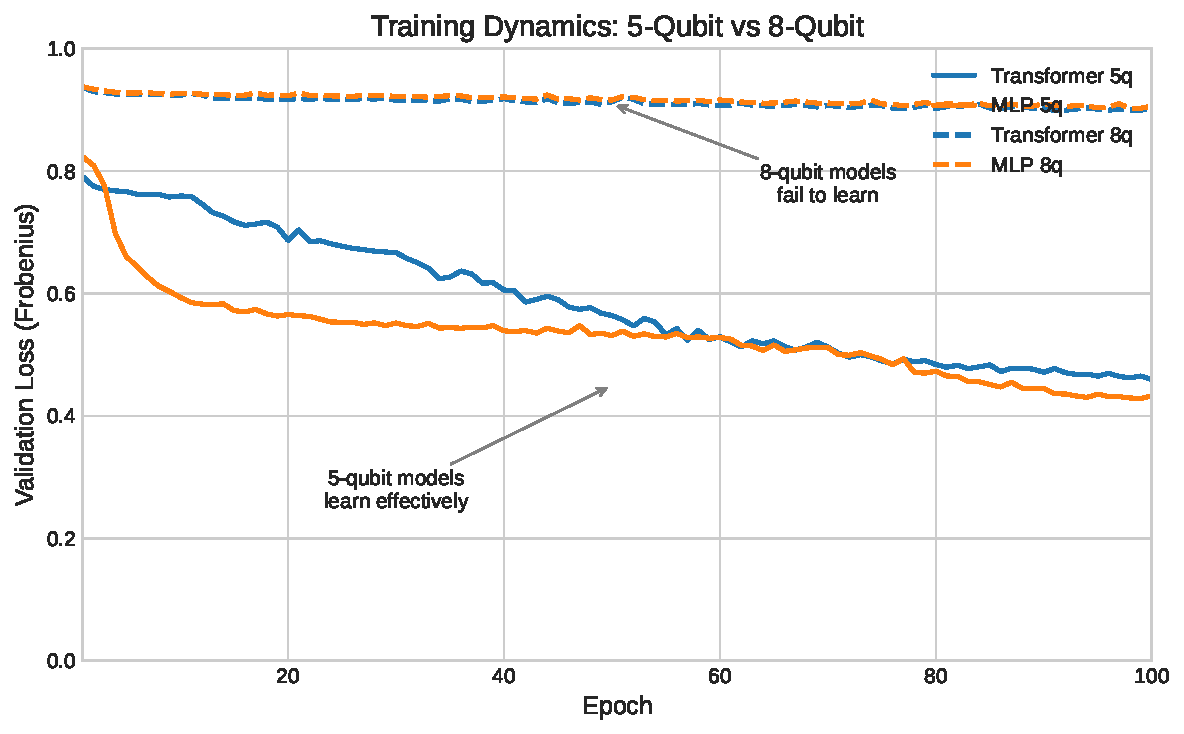
\includegraphics[width=.9\linewidth]{figures/val_loss_curves.pdf}
\caption{\label{fig:org696b6d3}Validation loss curves with Frobenius normalization. 5-qubit models (solid lines) show rapid initial improvement followed by gradual convergence. 8-qubit models (dashed lines) learn more slowly but maintain steady progress.}
\end{figure}

The 5-qubit curves show the expected pattern: rapid early improvement as models learn the dominant denoising structure, followed by gradual refinement. The 8-qubit curves progress more slowly, reflecting the massive increase in problem dimensionality, but crucially they \textbf{do} progress---in contrast to unnormalized training which plateaus immediately. To verify that stable convergence is not seed-dependent, we trained models with two additional random seeds; all runs converged to similar validation loss (see Appendix \ref{sec:org765c0e5}).

\section{Discussion}
\label{sec:org45e8c58}

\subsection{Why Normalization Matters}
\label{sec:orgb554cf7}

The physical origin of the scale mismatch is fundamental to quantum decoherence. The Frobenius norm of a density matrix equals the square root of its purity: \(\|\rho\|_F = \sqrt{\mathrm{Tr}(\rho^2)}\). Pure states have purity 1, while maximally mixed states have purity \(1/d\) (where \(d = 2^n\) for \(n\) qubits). Noise channels drive quantum states toward the maximally mixed state, systematically reducing their Frobenius norm.

For a 5-qubit system (\(d = 32\)), the maximally mixed state has \(\|\rho\|_F = 1/\sqrt{32} \approx 0.177\), giving a \textasciitilde{}5× scale gap from pure states. For 8 qubits (\(d = 256\)), this floor drops to \(1/\sqrt{256} = 0.0625\), a \textasciitilde{}16× gap. Our noisy states, driven toward the maximally mixed state by decoherence, have norms near these floors. This scale mismatch is not noise or measurement error; it is the physical signature of decoherence itself, and it grows exponentially with system size.

By normalizing to unit Frobenius norm, we remove this physically-determined but task-irrelevant scale variation, allowing models to focus on the coherence structure that distinguishes different quantum states.

\subsection{Architecture vs. Conditioning}
\label{sec:org6dd7f7d}

Our results highlight that input conditioning is more important than architectural choice for this task. With proper normalization:
\begin{itemize}
\item Both Transformer and MLP architectures achieve more than 3 times baseline improvement
\item Both architectures converge to similar final performance
\item Capacity scaling (width, depth) no longer hurts performance
\end{itemize}

The dramatic performance degradation observed in unnormalized capacity ablations (wide/deep MLPs performing 35\% worse than baseline) was due to optimization pathology caused by the scale mismatch, not fundamental model limitations.

\subsection{Numerical Precision}
\label{sec:org2add122}

Earlier experiments used single precision (float32), but we observed numerical instability when computing Uhlmann fidelity due to small negative eigenvalues arising from floating-point errors during eigendecomposition. Switching to double precision (float64) throughout the pipeline resolved these issues. We recommend float64 for quantum state computations where eigendecomposition is required (see Appendix \ref{sec:org85dfb55}).

\subsection{Hierarchical Tokenization}
\label{sec:orgd32645f}

For computational tractability at larger qubit counts, we use patch-based tokenization that maintains a fixed token count (64) regardless of system size. This trades spatial resolution for scalability:
\begin{itemize}
\item 5-qubit: \(4\times 4\) patches (32 complex values per patch)
\item 8-qubit: \(32\times 32\) patches (2048 complex values per patch)
\end{itemize}

The 8-qubit results validate this approach: despite extreme compression (2048:1), both models achieve more than 3 times baseline improvement. This would not have been possible without normalization enabling stable optimization in the first place.

\subsection{Limitations}
\label{sec:orgc54c349}

\subsubsection{Patch Size Ceiling}
\label{sec:org8903727}

Our 8-qubit results expose a fundamental limitation: when patches become too large (\(32\times 32\) = 2048 complex values), the information loss at embedding overwhelms any benefit from attention. The hierarchical approach requires patches small enough to preserve local structure while remaining computationally tractable.

For intermediate scales (6-7 qubits), smaller patches with more tokens may work---e.g., \(8\times 8\) patches on a \(64\times 64\) matrix yields 64 tokens with only 128 values per patch. We leave this exploration to future work.

\subsubsection{Noise Model Simplicity}
\label{sec:orgd84249a}

Our synthetic noise model assumes independent, Markovian noise channels acting on each qubit (depolarizing, amplitude damping, phase damping). Real quantum processors exhibit significant \textbf{crosstalk} (correlated errors between qubits) and \textbf{non-Markovian} memory effects. Extending our normalization approach to models trained on realistic correlated noise is an important direction for future work.

\subsubsection{Generalization to Real Hardware}
\label{sec:orgd88b9f5}

All experiments in this work rely on classical simulation of quantum states and noise. Deploying these models on actual hardware introduces challenges such as \textbf{calibration drift}, where the noise characteristics of the device change over time. A model trained on a static distribution of noise levels may degrade as the hardware drifts. Future work will investigate strategies for online adaptation or robust training across a wider envelope of noise parameters to mitigate this issue.

\subsubsection{Physical Constraints on Intermediate Representations}
\label{sec:org22209b6}

Our current approach enforces physical validity (Hermiticity, positive semi-definiteness, unit trace) only at evaluation time via post-hoc projection. An alternative would be to enforce these constraints on intermediate representations during training, potentially providing stronger inductive bias. However, our earlier experiments with Cholesky-constrained outputs---which guarantee valid density matrices by construction---caused models to collapse to trivial solutions (see Appendix, Failed Approaches). Future work could explore softer constraint mechanisms, such as physics-informed loss terms on intermediate layers or differentiable projections that maintain gradient flow while encouraging physically plausible representations throughout the network.

\section{Conclusion}
\label{sec:orga05145f}

We identify Frobenius normalization as a critical preprocessing step for training neural networks to denoise quantum density matrices. This simple technique---normalizing inputs and targets to unit Frobenius norm---addresses the fundamental scale mismatch between noisy and clean quantum states caused by decoherence.

\textbf{Key findings:}

\begin{enumerate}
\item \textbf{Normalization enables stable training.} Without normalization, models must simultaneously learn structural denoising and a large scale correction (\textasciitilde{}5× for 5 qubits, \textasciitilde{}16× for 8 qubits), leading to optimization pathology. Normalization improves validation loss by 25\% and enables stable convergence.

\item \textbf{Normalization enables scaling.} 8-qubit models (\(256\times 256\) matrices) fail completely without normalization but achieve 3.76 times baseline improvement with it. This demonstrates that normalization is not merely helpful but \textbf{essential} for scaling to larger quantum systems.

\item \textbf{Architecture-agnostic benefit.} Both Transformer and MLP architectures achieve similar performance with proper normalization, confirming that input conditioning is the critical factor for this task.

\item \textbf{Capacity ablations confirm the diagnosis.} Without normalization, wider (5 times) and deeper (2 times) MLPs perform \textbf{worse} than the baseline model---a clear signature of optimization pathology rather than underfitting.
\end{enumerate}

\textbf{Implications.} Our results suggest that future work on quantum state denoising should prioritize input conditioning over architectural innovation. The physical scale mismatch caused by decoherence is a domain-specific challenge that requires domain-specific preprocessing. We recommend Frobenius normalization as a standard preprocessing step for any neural approach to quantum state reconstruction.

\textbf{Future directions.} An intriguing finding is that the Transformer benefited more from normalization than the MLP (+25\% vs +11\% Uhlmann fidelity). We hypothesize that Transformers' internal LayerNorm operations may conflict with external scale mismatches: LayerNorm assumes inputs have consistent scale across the sequence, but unnormalized density matrices violate this assumption as different matrix regions have vastly different magnitudes depending on decoherence. Once external normalization resolves the scale mismatch, LayerNorm can function as intended. This suggests that architectures with internal normalization layers may be particularly sensitive to input preprocessing---and that other architectures previously dismissed for quantum tasks may warrant re-evaluation with proper conditioning.

\section{Acknowledgements}
\label{sec:org5965933}
The author used a large language model to edit parts of this work for clarity in presentation, and for debugging failed experiments and assisting with the code implementation. The technical content, experimental design, and interpretations are the author's own, and the author takes full responsibility for this work.
\section{Appendix}
\label{sec:orgedcb8b1}
\subsection{Model Parameter Counts}
\label{sec:orgcfbe387}
\begin{table}[htbp]
\caption{\label{tab:org6e3a21b}Detailed parameter breakdown.}
\centering
\begin{tabular}{lllll}
Component & 5-qubit Transformer & 8-qubit Transformer & 5-qubit MLP & 8-qubit MLP\\[0pt]
\hline
Patch embed & \(\sim 4\,\mathrm{k}\) & \(\sim 262\,\mathrm{k}\) & \(\sim 4\,\mathrm{k}\) & \(\sim 262\,\mathrm{k}\)\\[0pt]
Encoder & \(\sim 0.5\,\mathrm{M}\) & \(\sim 0.5\,\mathrm{M}\) & \(\sim 0.5\,\mathrm{M}\) & \(\sim 0.5\,\mathrm{M}\)\\[0pt]
Decoder & \(\sim 0.5\,\mathrm{M}\) & \(\sim 0.5\,\mathrm{M}\) & \(\sim 0.5\,\mathrm{M}\) & \(\sim 0.5\,\mathrm{M}\)\\[0pt]
Patch unembed & \(\sim 4\,\mathrm{k}\) & \(\sim 262\,\mathrm{k}\) & \(\sim 4\,\mathrm{k}\) & \(\sim 262\,\mathrm{k}\)\\[0pt]
Total & \(\sim 1.09\,\mathrm{M}\) & \(\sim 1.61\,\mathrm{M}\) & \(\sim 1.09\,\mathrm{M}\) & \(\sim 1.61\,\mathrm{M}\)\\[0pt]
\end{tabular}
\end{table}

\subsection{Frobenius vs. Uhlmann Correlation}
\label{sec:orga8b9d68}
To validate Frobenius fidelity as a training proxy, we analyzed its correlation with the ground-truth Uhlmann fidelity. Figure \ref{fig:orga5cfbc0} shows the relationship for 100 randomly sampled 5-qubit density matrices.

\begin{figure}[htbp]
\centering
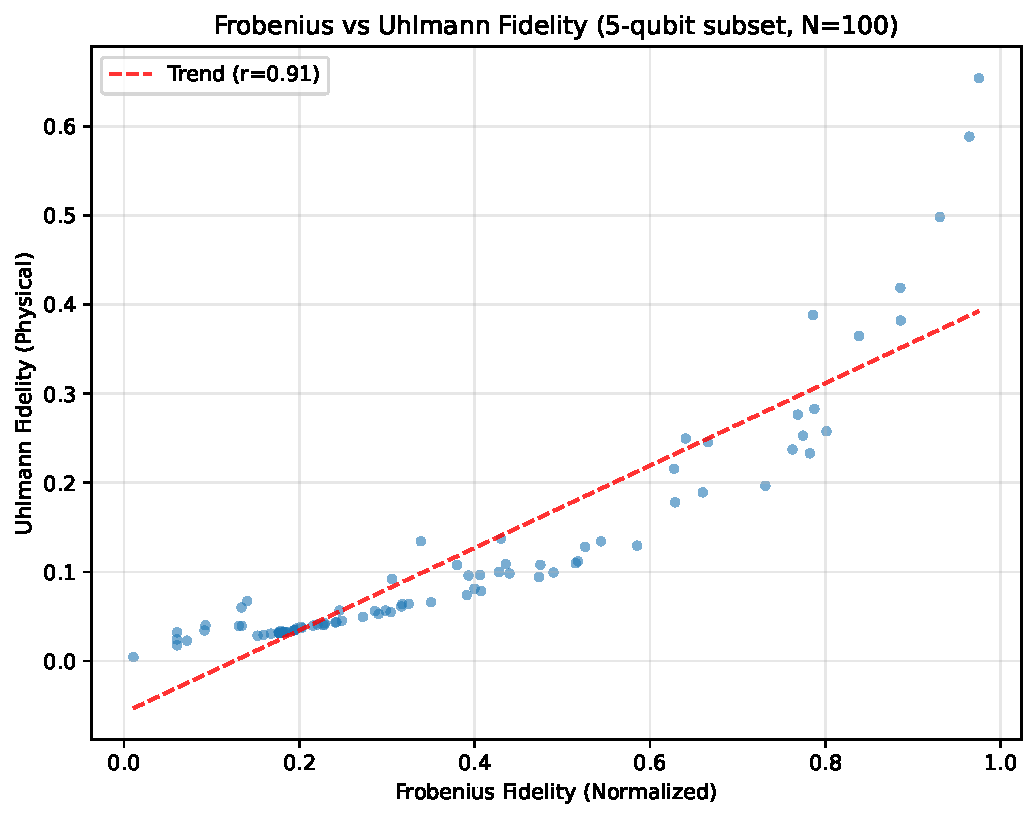
\includegraphics[width=.9\linewidth]{figures/frob_vs_uhlmann_correlation.pdf}
\caption{\label{fig:orga5cfbc0}Correlation between Frobenius fidelity (normalized) and Uhlmann fidelity (physical) on a random subset of the 5-qubit dataset. The strong correlation (\(r=0.91\)) justifies using Frobenius fidelity as a training proxy.}
\end{figure}

\subsection{Dataset}
\label{sec:org9c234f7}
\begin{table}[htbp]
\caption{\label{tab:orgc5ddd7b}Detailed parameter breakdown.}
\centering
\begin{tabular}{lll}
Trait & 5-qubit Dataset & 8-qubit Dataset\\[0pt]
\hline
Matrix size & 32 \texttimes{} 32 (1024 complex elements) & 256 \texttimes{} 256 (65,536 complex elements)\\[0pt]
Total samples & 100,000 & 100,000\\[0pt]
Precision & float64 & float64\\[0pt]
Storage & \(\sim\) 3.3 GB (preloaded into memory) & \(\sim\) 200 GB (streamed from disk)\\[0pt]
\end{tabular}
\end{table}


\subsection{Single vs Double Precision}
\label{sec:org85dfb55}
Early experiments used single precision (float32) for computational efficiency. However, we encountered numerical instability when computing Uhlmann fidelity, which requires eigendecomposition of density matrices. Small negative eigenvalues (order \(10^{-7}\) to \(10^{-8}\)) appeared due to floating-point accumulation errors, causing the square root operation in \(F(\rho, \sigma) = (\mathrm{Tr}[\sqrt{\sqrt{\rho}\sigma\sqrt{\rho}}])^2\) to produce NaN values.

Switching to double precision (float64) eliminated these issues. While this doubles memory usage and slightly increases computation time, the improved numerical stability is essential for reliable fidelity evaluation. All results in this paper use float64.

\subsection{Unnormalized Training Ablations}
\label{sec:org38fa73c}
The following ablations demonstrate the optimization pathology that occurs without Frobenius normalization. With unnormalized inputs (noisy matrices having \textasciitilde{}5× smaller norm than clean targets for 5-qubit systems), increasing model capacity \textbf{hurts} performance---a clear signature of optimization difficulties rather than underfitting.

\subsubsection{Capacity Ablation}
\label{sec:orgd4ef6ab}

We scaled MLP hidden dimensions by 4 times, increasing parameters from 1.09M to 5.29M.

\begin{table}[htbp]
\caption{\label{tab:org008af86}Capacity ablation without normalization: wider MLP performs worse, confirming optimization pathology.}
\centering
\begin{tabular}{llrl}
Model & Params & Uhlmann Fidelity & Notes\\[0pt]
\hline
MLP (matched) & 1.09M & 0.463 & Baseline MLP\\[0pt]
MLP (wide) & 5.29M & 0.310 & 5 times more params\\[0pt]
Transformer & 1.09M & 0.420 & Comparison\\[0pt]
\end{tabular}
\end{table}

The wide MLP performed 33\% \textbf{worse} than the matched MLP (0.310 vs 0.463), despite having nearly 5 times more parameters. This counter-intuitive result indicates severe optimization difficulties: the model has sufficient capacity but cannot find a good solution due to the ill-conditioned loss landscape.

\subsubsection{Depth Ablation}
\label{sec:org2ea8cca}

We doubled the number of layers from 4+4 to 8+8.

\begin{table}[htbp]
\caption{\label{tab:org7425f62}Depth ablation without normalization: deeper MLP performs worse, confirming optimization pathology.}
\centering
\begin{tabular}{lrlrl}
Model & Layers & Params & Uhlmann Fidelity & Notes\\[0pt]
\hline
MLP (matched) & 4+4 & 1.09M & 0.463 & Baseline MLP\\[0pt]
MLP (deep) & 8+8 & 2.15M & 0.407 & 2 times depth\\[0pt]
Transformer & 4+4 & 1.09M & 0.420 & Comparison\\[0pt]
\end{tabular}
\end{table}

The deep MLP performed 12\% \textbf{worse} than the matched MLP (0.407 vs 0.463). Together, these ablations confirm that the performance limitations in unnormalized training stem from optimization difficulties, not insufficient model capacity. With proper Frobenius normalization, the matched MLP improves from 0.463 to 0.516 Uhlmann fidelity.

\subsection{Seed Robustness}
\label{sec:org765c0e5}
To confirm that stable convergence under Frobenius normalization is not an artifact of a particular random initialization, we retrained 5-qubit models with two additional model initialization seeds (100 and 200) while keeping the data split fixed (seed=42).

\begin{center}
\begin{tabular}{rrr}
Init Seed & MLP Val Loss & Transformer Val Loss\\[0pt]
\hline
42 & 0.340 & 0.328\\[0pt]
100 & 0.337 & 0.347\\[0pt]
200 & 0.323 & 0.345\\[0pt]
\end{tabular}
\end{center}

ppAll runs converged to similar validation loss (0.32--0.35), confirming that normalization enables reproducible training across random initializations.

\subsection{Failed Approaches}
\label{sec:orgdf44f29}

During development, we explored several approaches that failed:

\begin{itemize}
\item \textbf{Cholesky output parameterization}: Constraining outputs to valid density matrices via Cholesky decomposition caused models to collapse to the maximally mixed state (I/d).
\item \textbf{Row-based tokenization}: Treating each matrix row as a token (32 tokens for 5-qubit) underperformed element-wise and patch-based approaches.
\item \textbf{Non-residual MLP}: Removing residual connections from the MLP caused catastrophic information loss, with performance worse than baseline.
\end{itemize}
\printbibliography
\end{document}
